\documentclass[./report.tex]{subfiles}
%\documentclass[../../../CR/pac.tex]{subfiles}

\begin{document}

\part{Monoserver Scheduling}

%% ===============================
\section{Principles for the implementation}
\label{sec:principles}

For all algorithms applied to single servers presented here the initial situation will be the same as illustrated here:
\begin{figure}[!h]
	\center
	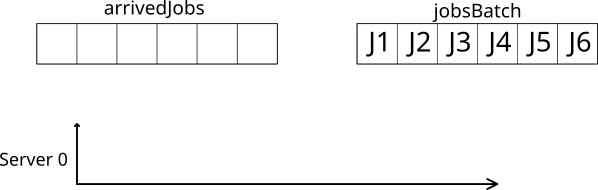
\includegraphics[scale=0.7]{part1/monoServer.png}
	\caption{Initial situation of a monoserver scheduling}
	\label{fig:monoServer_init} 
\end{figure}

We start with a jobs batch of loaded jobs from the test configuration file. A jobs batch is a list of jobs (or in our code a specialized class containing such a list). This jobs batch is sorted by order of arrivals. We initialize our scheduling algorithm by fetching the soonest jobs to arrive and adding them to the arrivedJobs list. We fetch the soonest jobs as we can't now for sure when is the first arrival date and how many jobs arrive at this same arrival dates.\\

Once the arrivedJobs list is initialized by fetching the soonest jobs to arrive we execute scheduling steps and we loop on these scheduling steps as long as the jobs batch and the arrivedJobs list aren't empty. A special case may happen at some point where the jobs batch isn't empty but the arrivedJobs is empty and the server isn't running any job. In this case we reinitialize our scheduling by fetching the soonest jobs to arrive again.\\

This common logic to all scheduling is what led us to implement this common loop used by all scheduling algorithms even in the next parts of this report:

\begin{lstlisting}[style=Java, caption={Main scheduling loop in Scheduler abstract class (cf. run() method)}]
protected void run(){
	while( !(jobsB.isEmpty() && arrivedJ.isEmpty() && serversM.areAllServersIdle()) ){
		if(serversM.areAllServersIdle() && arrivedJ.isEmpty()) arrivedJ.addAll(jobsB.getSoonestJobs());
		runScheduleStep();
	}
}
\end{lstlisting}

Another major principle of our scheduling algorithms used throughout all the exercises is the event-based system of scheduling steps. Instead of using time steps of 1 and checking at each time step the environment we use event steps. There are only two kinds of events we have to deal with so it is still easily manageable:
\begin{enumerate}
	\item A job has just finished
	\item A job has just arrived\\
\end{enumerate}

\newpage
Inside each schedule step we will have to compute the next event date based on these two possible events which is why we have the following method inside the Scheduler abstract class from which all scheduling algorithms inherit:
\begin{lstlisting}[style=Java, caption={Method used to compute the next event fate}]
protected double getNextEventDate(){
	double nextArrivalDate = jobsB.getNextArrivalDate();
	double nextJobToFinishDate = schedule.currentDate + serversM.getNextServerToFinish().getDuration();
	
	if(nextArrivalDate == -1) return nextJobToFinishDate;
	else return Math.min(nextArrivalDate, nextJobToFinishDate);
}
\end{lstlisting}

When an event occurs we will have to decide if an entry needs to be computed in the schedule\footnote{For example if a job has just finished or if it has been preempted} and by how much we have to decrement the currently running job's amount of units of work. We then fetch the jobs that have arrived in the meantime and we assign the newly arrived tasks to the server according to the specific algorithm assigning policy. Finally, we start another scheduling step which will "stop" when another another event occurs.\\

As you may notice even if all schedule steps have a common structure to manage the arrivedJobs list, the jobsBatch and also the current date of the schedule being computed, the further we get inside the schedule step the more it gets specific to the scheduling algorithm we choose. This is why the method \textit{runScheduleStep()} is abstract and is left to be redefined in each algorithm of this labwork.\\

Finally, we use a few helper classes such as the ServerManager class that provide functions to manage and observe the servers state through all the scheduling process. Which will lead us to use a few contractions:
\begin{itemize}
	\item serversM $\rightarrow$ serversManager as presented in section \ref{sec:principles}
	\item arrivedJ $\rightarrow$ arrivedJobs
	\item jobsB $\rightarrow$ jobsBatch\\
\end{itemize}

%% ===============================
\newpage
\section{FIFO}
\subsection{Implementation}

As the FIFO has been adapted to run on multiple servers, the \textit{decrementAll()} and \textit{assignArrivals()} methods take care of outputting entries in the Schedule object contained in the scheduler. One possible improvement on this labwork could be to further generalize the structure of a schedule step for all algorithms. Indeed, the illustrated code source will be very similar for all scheduling algorithms presented here.

\begin{lstlisting}[style=Java, caption={Source code of a FIFO schedule step}]
public void runScheduleStep() {
	if(serversM.areAllServersIdle() && !arrivedJ.isEmpty()){
		schedule.currentDate = arrivedJ.getFirst().getArrivalDate();
		serversM.initServers();
	}
	
	//We compute next event date:
	double nextEventDate = getNextEventDate();
	double unitsOfWorkDone = nextEventDate - schedule.currentDate;
	schedule.currentDate += unitsOfWorkDone;
	
	//We decrement and deal with finished jobs:
	serversM.decrementAll(unitsOfWorkDone);
	
	//We deal with new arrivals:
	arrivedJ.addAll(jobsB.getArrivedJobs(nextEventDate));
	assignArrivals();
}
\end{lstlisting}



\newpage
\subsection{Scheduling results}
\begin{figure}[!h]
	\center
	\includegraphics[scale=0.5]{test_monoServer_fifo.png}
	\caption{Output schedule produced by the FIFO scheduling algorithm on one server}
	\label{fig:monoServer_fifo} 
\end{figure}

Which corresponds to following file (<jobID, serverID, startDate, endDate, frequency>):
\lstinputlisting[style=txt, caption={Detail of the scheduling result}]{test_monoServer_fifo.txt}

\newpage
\subsection{Metrics}
\begin{lstlisting}[style=txt, caption={Metrics for FIFO on a single server}]
################ SCHEDULE METRICS ################

>> Scheduling Metrics: 
- Total Makespan: 126.0
- Nb Deadline Misses: 11
- Max Tardiness: 69.0
- Average Tardiness: 36.63636363636363
- Late Jobs: 
[Job: J6{6.0a/0.0u/30.0rd/36.0ad/100.0p} | Tardiness: 29.0 ]
[Job: J2{3.0a/0.0u/10.0rd/13.0ad/10.0p} | Tardiness: 8.0 ]
[Job: J2{13.0a/0.0u/10.0rd/23.0ad/10.0p} | Tardiness: 68.0 ]
[Job: J8{11.0a/0.0u/5.0rd/16.0ad/0.0p} | Tardiness: 64.0 ]
[Job: J4{5.0a/0.0u/30.0rd/35.0ad/0.0p} | Tardiness: 6.0 ]
[Job: J7{10.0a/0.0u/25.0rd/35.0ad/50.0p} | Tardiness: 40.0 ]
[Job: J7{60.0a/0.0u/25.0rd/85.0ad/50.0p} | Tardiness: 21.0 ]
[Job: J1{0.0a/0.0u/10.0rd/10.0ad/20.0p} | Tardiness: 5.0 ]
[Job: J5{6.0a/0.0u/12.0rd/18.0ad/0.0p} | Tardiness: 27.0 ]
[Job: J9{11.0a/0.0u/5.0rd/16.0ad/0.0p} | Tardiness: 69.0 ]
[Job: J1{20.0a/0.0u/10.0rd/30.0ad/20.0p} | Tardiness: 66.0 ]

>> Servers Metrics: 
- Servers work load:
Server #0 : 126.0

>> Energy Metrics: 
- Total Consumption: 2799.999999999995
- Max Consumption: 22.22222222222222
- Average Consumption: 2799.999999999995
- Consumption per Server: 
Server #0 : 2799.999999999995

##################################################
\end{lstlisting}


%% ===============================
\newpage
\section{Round Robin}
\subsection{Implementation}

Contrary to the FIFO algorithm which has been adapted to run on multiple servers this algorithm only works on a single server. One improvement on this labwork could be to develop a multiserver version of round robin.

\begin{lstlisting}[style=Java, caption={Source code of a Round Robin \textbf{on a single server} schedule step}]
	public void runScheduleStep() {
		Job job = arrivedJ.removeFirst();
		
		//We compute next event date:
		double start = ScheduleEntry.computeStart(schedule, serversM.getServers().getFirst(), job);
		double end = ScheduleEntry.computeEnd(job, start, QUANTUM);
		schedule.currentDate = end;
		
		//We decrement and deal with the finished job:
		job.decrement(QUANTUM);
		ScheduleEntry newEntry = new ScheduleEntry(job, serversM.getServers().getFirst(), start, end,
		serversM.getServers().getFirst().getCurrFreq());
		schedule.add(newEntry);
		
		//We deal with new arrivals:
		arrivedJ.addAll(jobsB.getArrivedJobs(end));
		if(!job.isWorkDone()) arrivedJ.add(job);
	}
\end{lstlisting}


\newpage
\subsection{Scheduling results}
\begin{figure}[!h]
	\center
	\includegraphics[scale=0.5]{test_monoServer_rr.png}
	\caption{Output schedule produced by the Round Robin scheduling algorithm on one server}
	\label{fig:monoServer_rr} 
\end{figure}

Which corresponds to following file (<jobID, serverID, startDate, endDate, frequency>):
\lstinputlisting[style=txt, caption={Detail of the scheduling result}]{test_monoServer_rr.txt}


\newpage
\subsection{Metrics}
\begin{lstlisting}[style=txt, caption={Metrics for Round Robin on a single server}]
################ SCHEDULE METRICS ################

>> Scheduling Metrics: 
- Total Makespan: 126.0
- Nb Deadline Misses: 13
- Max Tardiness: 70.0
- Average Tardiness: 43.07692307692308
- Late Jobs: 
[Job: J0{0.0a/0.0u/15.0rd/15.0ad/0.0p} | Tardiness: 48.0 ]
[Job: J9{11.0a/0.0u/5.0rd/16.0ad/0.0p} | Tardiness: 53.0 ]
[Job: J7{10.0a/0.0u/25.0rd/35.0ad/50.0p} | Tardiness: 55.0 ]
[Job: J5{6.0a/0.0u/12.0rd/18.0ad/0.0p} | Tardiness: 19.0 ]
[Job: J8{11.0a/0.0u/5.0rd/16.0ad/0.0p} | Tardiness: 52.0 ]
[Job: J1{0.0a/0.0u/10.0rd/10.0ad/20.0p} | Tardiness: 21.0 ]
[Job: J3{4.0a/0.0u/30.0rd/34.0ad/0.0p} | Tardiness: 48.0 ]
[Job: J4{5.0a/0.0u/30.0rd/35.0ad/0.0p} | Tardiness: 49.0 ]
[Job: J2{13.0a/0.0u/10.0rd/23.0ad/10.0p} | Tardiness: 48.0 ]
[Job: J1{20.0a/0.0u/10.0rd/30.0ad/20.0p} | Tardiness: 48.0 ]
[Job: J2{3.0a/0.0u/10.0rd/13.0ad/10.0p} | Tardiness: 32.0 ]
[Job: J6{6.0a/0.0u/30.0rd/36.0ad/100.0p} | Tardiness: 70.0 ]
[Job: J7{60.0a/0.0u/25.0rd/85.0ad/50.0p} | Tardiness: 17.0 ]

>> Servers Metrics: 
- Servers work load:
Server #0 : 126.0

>> Energy Metrics: 
- Total Consumption: 2799.999999999995
- Max Consumption: 22.22222222222222
- Average Consumption: 2799.999999999995
- Consumption per Server: 
Server #0 : 2799.999999999995

##################################################
\end{lstlisting}


%% ===============================
\newpage
\section{EDF}
\subsection{Implementation}
\label{subsec:edf}

Contrary to FIFO and round robin we notice that the arrived jobs list is now sorted based on a comparison key between jobs. For EDF this comparison key corresponds to the absolute deadline\footnote{arrival date + relative deadline of the job}. Also a jobs comparison predicate is used to allow us to compare two jobs (and not only a whole list) based on a criteria (which is still the absolute deadline here).
 
\begin{lstlisting}[style=Java, caption={Source code of an EDF schedule step}]
	protected void runScheduleStep() {
		arrivedJ.sort(JOBS_COMPARISON_KEY);
		if(serversM.areAllServersIdle() && !arrivedJ.isEmpty()){
			schedule.currentDate = arrivedJ.getFirst().getArrivalDate();
			serversM.initServers();
		}
		
		//We compute next event date:
		double nextEventDate = getNextEventDate();
		double unitsOfWorkDone = nextEventDate - schedule.currentDate;
		schedule.currentDate += unitsOfWorkDone;
		
		//We decrement and deal with finished jobs:
		serversM.decrementAll(unitsOfWorkDone);
		
		//We deal with new arrivals:
		arrivedJ.addAll(jobsB.getArrivedJobs(nextEventDate));
		arrivedJ.sort(JOBS_COMPARISON_KEY);
		assignArrivals(JOBS_COMPARISON_KEY, JOBS_COMPARISON_PREDICATE);
	}
\end{lstlisting}


\newpage
\subsection{Scheduling results}
\begin{figure}[!h]
	\center
	\includegraphics[scale=0.5]{test_monoServer_edf.png}
	\caption{Output schedule produced by the EDF scheduling algorithm on one server}
	\label{fig:monoServer_edf} 
\end{figure}

Which corresponds to following file (<jobID, serverID, startDate, endDate, frequency>):
\lstinputlisting[style=txt, caption={Detail of the scheduling result}]{test_monoServer_edf.txt}

\newpage
\subsection{Metrics}
\begin{lstlisting}[style=txt, caption={Metrics for EDF on a single server}]
################ SCHEDULE METRICS ################

>> Scheduling Metrics: 
- Total Makespan: 126.0
- Nb Deadline Misses: 11
- Max Tardiness: 60.0
- Average Tardiness: 23.363636363636363
- Late Jobs: 
[Job: J2{13.0a/0.0u/10.0rd/23.0ad/10.0p} | Tardiness: 18.0 ]
[Job: J6{6.0a/0.0u/30.0rd/36.0ad/100.0p} | Tardiness: 60.0 ]
[Job: J3{4.0a/0.0u/30.0rd/34.0ad/0.0p} | Tardiness: 22.0 ]
[Job: J5{6.0a/0.0u/12.0rd/18.0ad/0.0p} | Tardiness: 17.0 ]
[Job: J0{0.0a/0.0u/15.0rd/15.0ad/0.0p} | Tardiness: 6.0 ]
[Job: J9{11.0a/0.0u/5.0rd/16.0ad/0.0p} | Tardiness: 15.0 ]
[Job: J7{60.0a/0.0u/25.0rd/85.0ad/50.0p} | Tardiness: 21.0 ]
[Job: J4{5.0a/0.0u/30.0rd/35.0ad/0.0p} | Tardiness: 31.0 ]
[Job: J8{11.0a/0.0u/5.0rd/16.0ad/0.0p} | Tardiness: 10.0 ]
[Job: J7{10.0a/0.0u/25.0rd/35.0ad/50.0p} | Tardiness: 41.0 ]
[Job: J1{20.0a/0.0u/10.0rd/30.0ad/20.0p} | Tardiness: 16.0 ]

>> Servers Metrics: 
- Servers work load:
Server #0 : 126.0

>> Energy Metrics: 
- Total Consumption: 2799.999999999995
- Max Consumption: 22.22222222222222
- Average Consumption: 2799.999999999995
- Consumption per Server: 
Server #0 : 2799.999999999995

##################################################
\end{lstlisting}


%% ===============================
\newpage
\section{RMS}
\subsection{Implementation}
\label{subsec:rms}

As mentioned in the previous subsection \ref{subsec:edf} on the EDF implementation the algorithm is basically the same. Only the comparison keys and predicates change. Indeed, in EDF we have the following comparison keys/predicates: 

\begin{lstlisting}[style=Java, caption={Comparison key and predicate of EDF}]
	private static final Comparator<Job> JOBS_COMPARISON_KEY = Comparator.comparingDouble(Job::getADeadline);
	private static final BiPredicate<Job, Job> JOBS_COMPARISON_PREDICATE = (Job j1, Job j2) -> j1.getADeadline() < j2.getADeadline();
\end{lstlisting}

While on RMS we have the more complex ones here:
\begin{lstlisting}[style=Java, caption={Comparison key and predicate of RMS}]
	private static final Comparator<Job> JOBS_COMPARISON_KEY = (j1, j2) -> {
		if (j1.getPeriod() == j2.getPeriod())
		return Double.compare(j1.getADeadline(), j2.getADeadline());
		else
		return Double.compare(j1.getPeriod(), j2.getPeriod());
	};
	private static final BiPredicate<Job, Job> JOBS_COMPARISON_PREDICATE =  (j1, j2) -> {
		if (j1.getPeriod() == j2.getPeriod())
		return j1.getADeadline() <= j2.getADeadline();
		else
		return j1.getPeriod() <= j2.getPeriod();
	};
\end{lstlisting}

This comparison key/predicate for RMS allows us to first sort/compare the tasks using their period (smallest periods being the most important) then, if the jobs are without periods (period = 0), to sort/compare them according to their absolute deadlines (just like with EDF).

\newpage
\subsection{Scheduling results}
\begin{figure}[!h]
	\center
	\includegraphics[scale=0.5]{test_monoServer_rms.png}
	\caption{Output schedule produced by the RMS scheduling algorithm on one server}
	\label{fig:monoServer_rms} 
\end{figure}

Which corresponds to following file (<jobID, serverID, startDate, endDate, frequency>):
\lstinputlisting[style=txt, caption={Detail of the scheduling result}]{test_monoServer_rms.txt}

\newpage
\subsection{Metrics}
\begin{lstlisting}[style=txt, caption={Metrics for RMS on a single server}]
################ SCHEDULE METRICS ################

>> Scheduling Metrics: 
- Total Makespan: 126.0
- Nb Deadline Misses: 8
- Max Tardiness: 71.0
- Average Tardiness: 50.25
- Late Jobs: 
[Job: J4{5.0a/0.0u/30.0rd/35.0ad/0.0p} | Tardiness: 71.0 ]
[Job: J1{0.0a/0.0u/10.0rd/10.0ad/20.0p} | Tardiness: 1.0 ]
[Job: J6{6.0a/0.0u/30.0rd/36.0ad/100.0p} | Tardiness: 16.0 ]
[Job: J8{11.0a/0.0u/5.0rd/16.0ad/0.0p} | Tardiness: 61.0 ]
[Job: J5{6.0a/0.0u/12.0rd/18.0ad/0.0p} | Tardiness: 68.0 ]
[Job: J9{11.0a/0.0u/5.0rd/16.0ad/0.0p} | Tardiness: 66.0 ]
[Job: J0{0.0a/0.0u/15.0rd/15.0ad/0.0p} | Tardiness: 57.0 ]
[Job: J3{4.0a/0.0u/30.0rd/34.0ad/0.0p} | Tardiness: 62.0 ]

>> Servers Metrics: 
- Servers work load:
Server #0 : 126.0

>> Energy Metrics: 
- Total Consumption: 2799.999999999995
- Max Consumption: 22.22222222222222
- Average Consumption: 2799.999999999995
- Consumption per Server: 
Server #0 : 2799.999999999995

##################################################
\end{lstlisting}


%% ===============================
\newpage
\section{Comparison Table}

\begin{tabular}{|m{8em}|m{12em}|m{12em}|m{12em}|} 
	\hline 
	\textbf{Algorithm} & \textbf{Pros} & \textbf{Cons} & \textbf{Possible Uses} \\ 
	\hline
	FIFO 
	&  
	\begin{itemize}[leftmargin=*]
		\item Easy to implement and debug
		\item Corresponds to the expected behavior of many applications (e.g. printers, chains of tasks such as piped commands, etc.)
	\end{itemize}
	&  
	\begin{itemize}[leftmargin=*]
		\item Risks of starvation if a task is blocked
		\item Risks of heavy tardiness if a task takes an exceptionally long amount of time to complete
	\end{itemize}
	& 
	\begin{itemize}[leftmargin=*]
		\item When the application requires tasks to execute in a consecutive order (could be made safer with a timeout mechanic)
	\end{itemize}
	\\
	\hline
	Round Robin 
	&  
	\begin{itemize}[leftmargin=*]
		\item Prevents starvation
		\item Still rather easy to implement and debug
	\end{itemize}
	&  
	\begin{itemize}[leftmargin=*]
		\item Tends to even more increase the number of deadline misses and average tardiness of tasks if the quantum is short
	\end{itemize}
	& 
	\begin{itemize}[leftmargin=*]
		\item With a reasonable quantum and if a strict sequence in the order of treated tasks isn't needed as in FIFO, it can be a fair way to run tasks while being starvation-free.
	\end{itemize}
	\\
	\hline
	EDF 
	&  
	\begin{itemize}[leftmargin=*]
		\item Lowest tardiness of tasks (but not necessarily lowest number of deadline misses)
	\end{itemize}
	&  
	\begin{itemize}[leftmargin=*]
		\item A bit more complex to implement and maintain
		\item Not starvation free as if no new arrival with higher priority comes then priorities are fixed and a blocked running task can block all the other tasks
	\end{itemize}
	& 
	\begin{itemize}[leftmargin=*]
		\item Useful if we want highly responsive applications
	\end{itemize}
	\\
	\hline
	RMS 
	&  
	\begin{itemize}[leftmargin=*]
		\item Lowest number of deadline misses
	\end{itemize}
	&  
	\begin{itemize}[leftmargin=*]
		\item  A bit more complex to implement and maintain (but once you have implemented EDF it's rather straightforward and reciprocally)
		\item Not starvation free for the same reasons than with EDF
	\end{itemize}
	& 
	\begin{itemize}[leftmargin=*]
		\item Probably the best algorithm for hard real-time operating systems where deadline misses isn't an option
	\end{itemize}
	\\
	\hline
\end{tabular}

\end{document}